% L13a figure: the four pieces of a URL.
%
% The URL is the hourly forecast for Ithaca, NY from the National Weather
% Service API, in metric units. A bracket marks each piece: the scheme, the
% host, the path, and the query string. Blue marks the piece names.
%
% Drawn on November 12, 2026 with the palette and build of the L12c figures.
% The notebook SVG carries a dark palette added by theme_svg.py; keep new colors
% in that script's mapping when changing the palette here.
\documentclass[tikz,border=4pt]{standalone}
\usepackage[no-math]{fontspec}
\IfFontExistsTF{Arial}{\setsansfont{Arial}}{\setsansfont{TeX Gyre Heros}}
\IfFontExistsTF{Menlo}{\setmonofont{Menlo}[Scale=0.88]}{}
\renewcommand{\familydefault}{\sfdefault}
\usepackage{amsmath,amssymb}
\usetikzlibrary{arrows.meta, calc, fit, backgrounds, positioning, decorations.pathreplacing}

% Ink, blue, gray, and band match the L12c figures.
\definecolor{vnink}{HTML}{202124}
\definecolor{gdblue}{HTML}{0091FF}
\definecolor{gdgray}{HTML}{6D7278}
\definecolor{waband}{HTML}{EEF0F2}
\definecolor{nodefill}{HTML}{FFFFFF}

\begin{document}
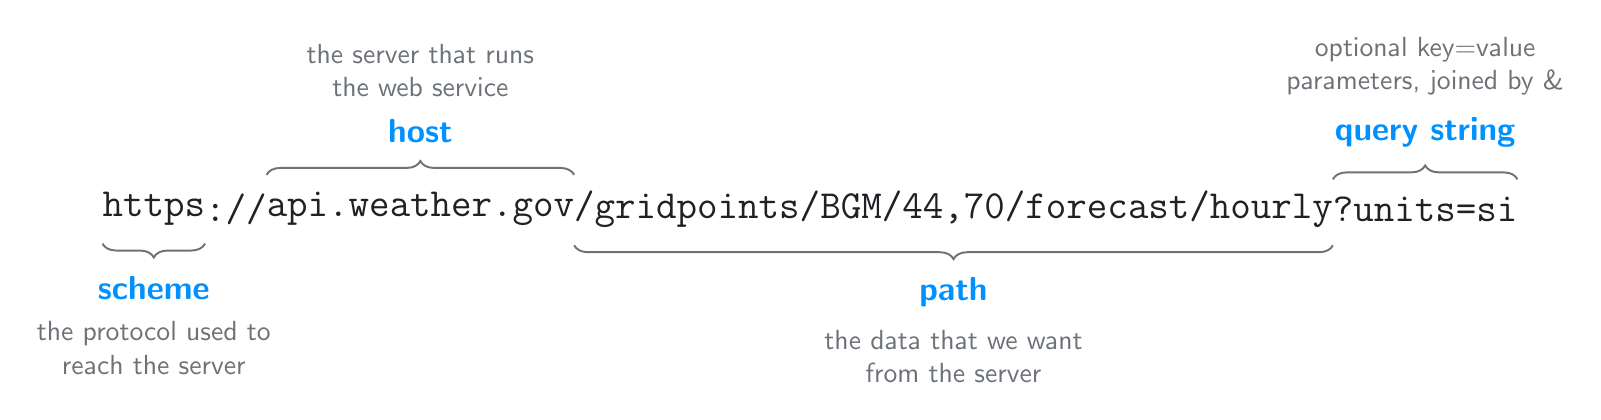
\begin{tikzpicture}[
  font=\sffamily\large,
  piece/.style={font=\ttfamily\Large, text=vnink, inner xsep=0pt, inner ysep=5pt, outer sep=0pt},
  pname/.style={font=\sffamily\large\bfseries, text=gdblue, align=center},
  what/.style={font=\sffamily\normalsize, text=gdgray, align=center},
  br/.style={decorate, decoration={brace, amplitude=5pt}, draw=gdgray, line width=0.7pt}
]
\node[piece] (scheme) at (0,0) {https};
\node[piece, right=0pt of scheme] (sep) {://};
\node[piece, right=0pt of sep] (host) {api.weather.gov};
\node[piece, right=0pt of host] (path) {/gridpoints/BGM/44,70/forecast/hourly};
\node[piece, right=0pt of path] (query) {?units=si};

% scheme and path are labeled below, host and query string above
\draw[br] ($(scheme.south east)+(0,-0.05)$) -- ($(scheme.south west)+(0,-0.05)$)
  node[pname, midway, below=8pt] (ns) {scheme};
\node[what, below=1pt of ns] {the protocol used to\\reach the server};

\draw[br] ($(host.north west)+(0,0.05)$) -- ($(host.north east)+(0,0.05)$)
  node[pname, midway, above=8pt] (nh) {host};
\node[what, above=1pt of nh] {the server that runs\\the web service};

\draw[br] ($(path.south east)+(0,-0.05)$) -- ($(path.south west)+(0,-0.05)$)
  node[pname, midway, below=8pt] (np) {path};
\node[what, below=1pt of np] {the data that we want\\from the server};

\draw[br] ($(query.north west)+(0,0.05)$) -- ($(query.north east)+(0,0.05)$)
  node[pname, midway, above=8pt] (nq) {query string};
\node[what, above=1pt of nq] {optional key=value\\parameters, joined by \&};

\end{tikzpicture}
\end{document}
